\documentclass[11pt]{article}

\usepackage{amsmath,amssymb}

\usepackage[letterpaper, margin=1in]{geometry}
\usepackage{listings}

\usepackage[final]{graphicx}
\usepackage{hyperref}
\allowdisplaybreaks

\usepackage{float}
\usepackage{multicol}
% Comment the following line to use TeX's default font of Computer Modern.
\usepackage{times,txfonts}
\usepackage{mwe}
\usepackage{caption}
\usepackage{subcaption}

\begin{document}

\title{Graph Diffusion}

\author{Stefano Fochesatto}

\date{\today}

\maketitle

\section{Introduction}  
Throughout our course we have considered the heat equation for many examples; simple 
problems with square boundaries and straight forward discretization schemes. The goal of this project
is to study diffusion equation with graphs as the domain. 

This problem can be thought of as a continuous version of the network flow problems discussed in optimization. 
Suppose there exists some flow, in most examples we've seen that flow represents heat and in the context of optimization
goal was to move flow from one vertex to another in an underlying network as efficiently as possible. Here 
our goal is to model the state of this flow as a closed system which respects conservation laws. 

% introduce weighted degree
% Weighted adjacency 
% Definition of graph laplacian
% Undirected graphs. 










%PUT CONTENT HERE; PERHAPS CITE SOMETHING \cite{einstein}

%\begin{figure}
%\includegraphics[width=0.5\textwidth]{foo.png}  % put image "foo.png" in current directory
%\caption{CAPTION TEXT HERE}
%\end{figure}

\section{Continuum Model [or Continuum Problem]} 
For this problem we will be considering weighted undirected graphs. 
We let each vertex be denoted by $v_i$, weighted edge by $\omega_{ij}$, and flow (heat) at a vertex by $\phi_i$. By Newton's law of cooling, applied 
between two vertices $v_i$ and $v_j$ we can model the change in flow from $v_i$ to $v_j$ by the following, 
\begin{equation*}
    \dfrac{\partial \phi_{ij}}{\partial t} = \alpha \omega_{ij}(\phi_i(t) - \phi_j(t)).
\end{equation*}
Note that when $\phi_i(t)>\phi_j(t)$, this quantity is positive and therefore ascribes a positive sign to heat leaving $v_i$. 
Describing the change in flow at a single vertex $v_i$ requires us to sum the previous relation across all vertices in the neighborhood of $v_i$. Note that 
inverting the sign on the sum gives us a negative quantity when flow is leaving the vertex. 
Doing so we get the following, 
\begin{equation*}
    \dfrac{\partial \phi_{i}}{\partial t} = -\sum_{j: v_j \in \mathcal{N}(v_i)} \alpha \omega_{ij}(\phi_i(t) - \phi_j(t)).
\end{equation*}





This results in a system of coupled differential equations, defined by the paths in the graph. Consider small, three vertex path $v_a$, $v_b$, $v_c$
and suppose $v_c \not\in \mathcal{N}(v_a)$. Note that since $v_b \in \mathcal{N}(v_a), \mathcal{N}(v_c)$ we have the following equations, 
\begin{align*}
    \dfrac{\partial \phi_{a}}{\partial t} &= -\sum_{j: v_j \in \mathcal{N}(v_a)} \alpha \omega_{ij}(\phi_i(t) - \phi_j(t))\\ 
    &= -\alpha\omega_{ab}(\phi_a(t) - \phi_b(t)) - \left(\sum_{j: v_j \in \mathcal{N}(v_a)\setminus\{v_b\}} \alpha \omega_{aj}(\phi_a(t) - \phi_j(t))\right),
\end{align*}  
\begin{align*}
    \dfrac{\partial \phi_{c}}{\partial t} &= -\sum_{j: v_j \in \mathcal{N}(v_c)} \alpha \omega_{ij}(\phi_i(t) - \phi_j(t))\\
    &= -\alpha\omega_{cb}(\phi_c(t) - \phi_b(t)) - \left(\sum_{j: v_j \in \mathcal{N}(v_c)\setminus\{v_b\}} \alpha \omega_{cj}(\phi_c(t) - \phi_j(t))\right).
\end{align*}  
Since $\phi_b(t)$ is contained in both equations we can write $\dfrac{\partial \phi_{a}}{\partial t}$ with respect to $\phi_c$ and  $\dfrac{\partial \phi_{a}}{\partial t}$, and a similar substitution can be extended to 
paths of arbitrary length. Physically this means that the coupled nature of our system is modeling the fact that flow is moving across path connected vertices not just adjacent vertices. 




Since we are working with a weighted undirected graph, in the context of this problem the adjacency and degree matrices are weighted. So the adjacency matrix
is filled with the corresponding $\omega_{ij}$, and the degree matrix can just be thought of as a diagonal matrix where the diagonal is a column or row sum of the adjacency.  
Therefore an edge weighted sum over the neighborhood of a vertex $v_i$ can be described with the $i^{th}$ row of the adjacency matrix like so, 
\begin{equation*}
    \dfrac{\partial \phi_{i}}{\partial t} = -\sum_{j: v_j \in \mathcal{N}(v_i)} \alpha \omega_{ij}(\phi_i(t) - \phi_j(t)) =  -\alpha \sum_{j = 1}^n A_{ij}(\phi_i(t) - \phi_j(t))
\end{equation*} 


Note that the graph Laplacian is defined by $L = D - A$, where $D$ and $A$ are the weighted adjacency and degree matrices we've been working with.\cite{spielman}
With some further algebraic manipulation we find that this whole computation can be written in terms of the graph Laplacian matrix, 
\begin{align*}
    \dfrac{\partial \phi_{i}}{\partial t} &= -\alpha \sum_{j = 1}^n A_{ij}(\phi_i(t) - \phi_j(t))\\
    &= -\alpha \left(\sum_{j = 1}^n A_{ij}\phi_i(t) + \sum_{j = 1}^n A_{ij} \phi_j(t)\right)\\
    &= -\alpha \left(\phi_i(t) \sum_{j = 1}^n A_{ij} + \sum_{j = 1}^n A_{ij} \phi_j(t)\right)\\
    &= -\alpha \left(\deg(\phi_i)\phi_i(t) + \sum_{j = 1}^n A_{ij} \phi_j(t)\right)\\
    &= -\alpha \sum_{j = 1}^n (\delta_{ij}\deg(\phi_i) - A_{ij}) \phi_j(t)
\end{align*}
Where $\delta_{ij}$ denotes the kronecker delta function, allowing us to represent an entire row of the graph Laplacian matrix with a single sum. 
When applied to every vertex in the graph, we form a column vector of flow, $\phi(t)$ and arrive at the formulation of our problem.\cite{Simon}
\begin{equation*}
    \dfrac{\partial \phi}{\partial t} = -\alpha L \phi(t).
\end{equation*}





\subsection*{Connection to the $\nabla^2$ Operator}
Interestingly this problem can be seen as a more general discretization stencil for an arbitrary dimension Laplacian. We can see this by considering the following 
reformulation of $\dfrac{\partial \phi_{i}}{\partial t}$,
\begin{align*}
    \dfrac{\partial \phi_{i}}{\partial t} &= -\sum_{j: v_j \in \mathcal{N}(v_i)} \alpha \omega_{ij}(\phi_i(t) - \phi_j(t))\\
         &= -\sum_{j: v_j \in \mathcal{N}(v_i)} \alpha \omega_{ij}(\phi_i(t) - \phi_j(t))\\
         &= -\alpha \left(\phi_i(t) \sum_{j: v_j \in \mathcal{N}(v_i)}\omega_{ij} + \sum_{j: v_j \in \mathcal{N}(v_i)}\omega_{ij}\phi_j(t)\right) \\
         &= \alpha \left(\sum_{j: v_j \in \mathcal{N}(v_i)}\omega_{ij}\right) \left(\dfrac{\sum_{j: v_j \in \mathcal{N}(v_i)}\omega_{ij}\phi_j(t)}{ \sum_{j: v_j \in \mathcal{N}(v_i)}\omega_{ij}} - \phi_i(t)\right)
\end{align*}
Now consider the 5-point stencil for the Laplacian in two spatial dimensions with a constant diffusivity coefficient i.e. $\alpha \nabla^2$. Recall that using centered finite differences results in the following 
approximation of the Laplacian at a point $u_{i, j}$,\cite{leveque} 
\begin{equation*}
    \alpha\nabla^2(u_{i, j}) = \alpha\frac{4}{h^2}\left(\dfrac{u_{i - 1, j} + u_{i + 1, j} + u_{i, j-1} + u_{i, j+1}}{4} - u_{i, j}\right).
\end{equation*}
This stencil resembles a row of the graph Laplacian corresponding to a vertex with 4 neighbors, where the weights $\omega_j$ have all been forced to $1/h^2$.
Here, adding more spatial dimensions to the Laplacian would correspond to a vertex with more neighbors, and incorporating unequal spacing would force unequal weights. 

\subsection*{Analytical Solution}

First we will show that the graph Laplacian $L$ is positive semi-definite. Showing this, along with the fact that $L$ is symmetric would imply that 
$L$ has real, non-negative eigenvalues. We proceed by considering the following, let $\phi \in \mathbb{R}^n$ and consider $\phi^TL\phi$. From our previous computations we know 
that the $i^{th}$ term in $(L\phi)$ contains a sum over the corresponding row in the adjacency matrix $A$. We consider computing $\phi^T(L\phi)$ entry-wise and by substitution we get the following, 
\begin{align*}
    \phi^TL\phi &= \sum_{i = 1}^n \phi_i (L\phi)_i\\
     &= \sum_{i = 1}^n \phi_i \left(\sum_{j = 1}^n A_{ij}(\phi_i - \phi_j)\right)\\
     &= \sum_{i = 1}^n \sum_{j = 1}^n A_{ij}(\phi_i^2 - \phi_i\phi_j)\\
     &= \frac{2}{2}\sum_{i = 1}^n \sum_{j = 1}^n A_{ij}(\phi_i^2 - \phi_i\phi_j)\\
     &= \frac{1}{2}\sum_{i = 1}^n \sum_{j = 1}^n A_{ij}2(\phi_i^2 - \phi_i\phi_j)\\
     &= \frac{1}{2}\sum_{i = 1}^n \sum_{j = 1}^n A_{ij}(\phi_i^2 - 2\phi_i\phi_j + \phi_i^2)
\end{align*}
Now note that by switching the order of the sums, swapping the indexing variables, and applying the fact that $A$ is a symmetric matrix we get, 
\begin{equation*}
    \sum_{i = 1}^n\sum_{j = 1}^n A_{ij}(\phi_i^2) =
    \sum_{j = 1}^n\sum_{i = 1}^n A_{ij}(\phi_i^2) =
    \sum_{j = 1}^n\sum_{i = 1}^n A_{ji}(\phi_j^2) =
    \sum_{j = 1}^n\sum_{i = 1}^n A_{ij}(\phi_j^2).
\end{equation*}
So by substitution we get the following, 
\begin{align*}
     &= \frac{1}{2}\sum_{i = 1}^n \sum_{j = 1}^n A_{ij}(\phi_i^2 - 2\phi_i\phi_j + \phi_j^2),\\
     &= \frac{1}{2}\sum_{i = 1}^n \sum_{j = 1}^n A_{ij}(\phi_i - \phi_j)^2.
\end{align*}
Note that this computation becomes a weighted sum of square differences across all adjacent vertices which will always be greater than or equal to zero. Therefore 
we conclude that $\phi^TL\phi \geq 0$ and $L$ is positive semi-definite. 

An even stronger result states that $\lambda_1 = 0$ with multiplicity equal to the number of connected components of the graph, and that the first non-null
eigenvalue (Fiedler Value) is a measure of how connected the graph is.\cite{Poignard} 



We also find that for connected graphs, like the one in question the eigenvectors form an 
orthonormal basis.\cite{Radu}

%https://csustan.csustan.edu/~tom/Clustering/GraphLaplacian-tutorial.pdf
%file:///Users/stefanofochesatto/Downloads/GenericLaplacians_preprint.pdf



Finally we formulate the analytical solution, in the same way we would construct a solution for a system of ODE using the matrix exponential. Let 
$\eta = \phi(0)$, and since $L$ is diagonalizable with $|\lambda_i| \geq 0$ since it is SPD, and with orthogonal eigenvectors we get the following, 
\begin{equation*}
    \phi(t) = Re^{-\alpha \Lambda t}R^T\eta.
\end{equation*}






%\begin{equation*}
   % \dfrac{\partial \phi_{a}}{\partial t} =  -\alpha\omega_{ab}(\phi_a(t) -  \dfrac{1}{\alpha\omega_{cb}}\left(\dfrac{\partial \phi_{c}}{\partial t} + \left(\sum_{j: v_j \in \mathcal{N}(v_c)\setminus\{v_b\}} \alpha \omega_{ij}(\phi_i(t) - \phi_j(t))\right) + \phi_c(t)\right)    ) - \left(\sum_{j: v_j \in \mathcal{N}(v_a)\setminus\{v_b\}} \alpha \omega_{ij}(\phi_i(t) - \phi_j(t))\right)
%\end{equation*}





\section{Numerical Scheme(s)} 
As stated this problem is a system of ODE IVP, and therefore an application of any of the ODE IVP schemes discussed 
throughout the course would be suitable. As we have previously mentioned, the first non-null eigenvalue of the Laplacian (Fiedler Value)
gives a measurement of how well connected the graph is. For our connected graph we know that $\lambda_1 = 0$ and since our eigenvalues 
are all real, the stiffness ratio of $L$ will actually be a useful measure of stiffness. Since the stiffness ratio will be at least as large as
$\lambda_2$, it follows that for highly connected graphs this problem becomes stiff. 


For our numerical analysis portion of this project we will proceed on two variation of this problem, a minimally connected graph and a highly connected graph
applying both forward and backward Euler. 

The following are the codes for implementing forward and backward Euler on this system. \\

\textbf{Code:}
\begin{center}
    \lstinputlisting[basicstyle=\footnotesize]{r1.txt}
\end{center}

\textbf{Code:}
\begin{center}
    \lstinputlisting[basicstyle=\footnotesize]{r2.txt}
\end{center}



\section{Analysis} 
For the analysis I generated two random graphs on 10 vertices. Both graphs where forced to be connected, and the weights $\omega_i$ were chosen from 
a normal distribution with $\mu = 0$ and $\sigma = 4$ then the the absolute value was taken. Connectivity was controlled using 
samples from a uniform distribution. The following are the graphs that were generated for the convergence analysis, 

\begin{figure}[H]
    \begin{center}
        \caption{Low Connectivity Graph. Edge weights $\omega_i$ are shown.}
      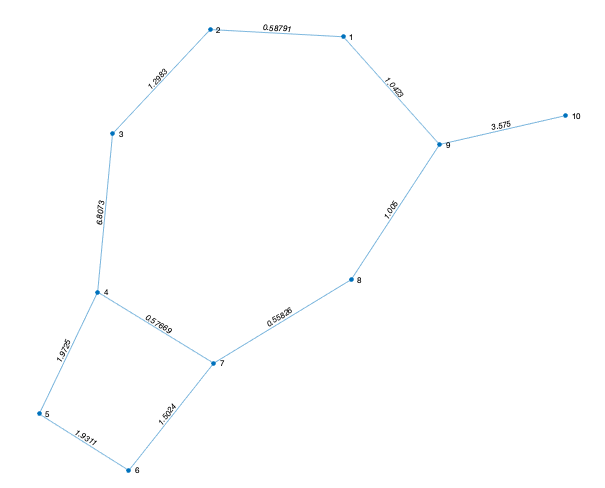
\includegraphics[width=.60\textwidth]{GLowGraph.png}
    \end{center}
  \end{figure}


\begin{figure}[H]
    \begin{center}
        \caption{High Connectivity Graph. Edge weights $\omega_i$ are omitted.}
      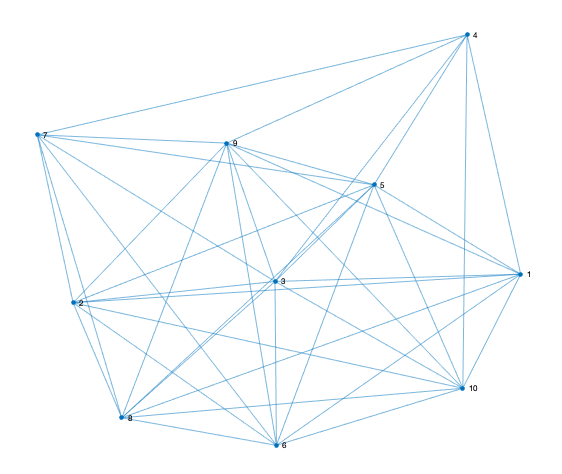
\includegraphics[width=.60\textwidth]{GHighGraph.png}
    \end{center}
  \end{figure}


Here is all the code used to run the convergence analysis and generate these graphs.\\

\textbf{Code:}
\begin{center}
    \lstinputlisting[basicstyle=\footnotesize]{r3.txt}
\end{center} 

\section{Results}  
For the convergence analysis we used a refinement grid of $N = [10, 100, 1000, 10000, 100000]$, a one hot initial value $\eta$ and a 
$t_f = 1$. Below is a comparison of the convergence of $t_f$ of the two graphs using forward Euler, 

\begin{figure}[H]
    \begin{center}
      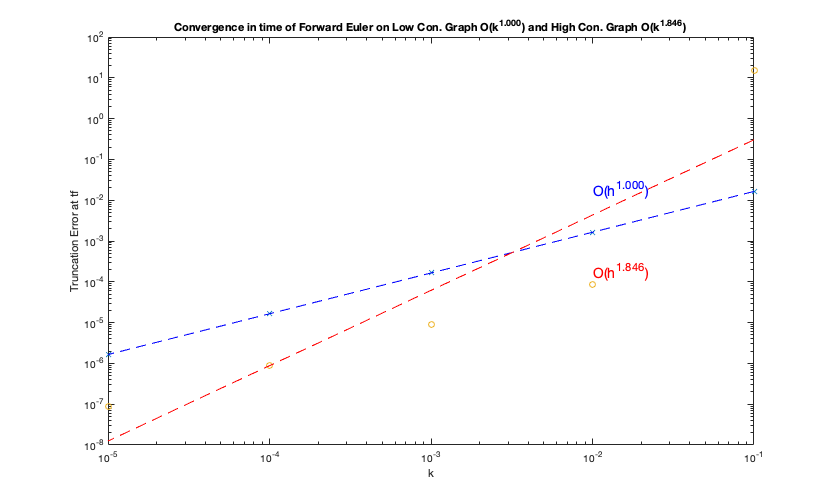
\includegraphics[width=\textwidth]{ForwardEuler.png}
    \end{center}
  \end{figure}

This analysis showed that for the higher connectivity graph the convergence was better. Looking at the eigenvalues of the graph Laplacians
we find that the higher connectivity graph has a larger eigenvalue by a magnitude of 3,\\

\textbf{Console:}
\begin{center}
    \lstinputlisting[basicstyle=\footnotesize]{r4.txt}
\end{center} 

Despite the higher connectivity graph producing a more stiff problem, it's convergence rate, using forward Euler was faster than the less 
stiff problem produced by the lower connectivity graph. 



The backward Euler scheme produced a more expected result, but still the higher connectivity graph has faster convergence. 
\begin{figure}[H]
    \begin{center}
      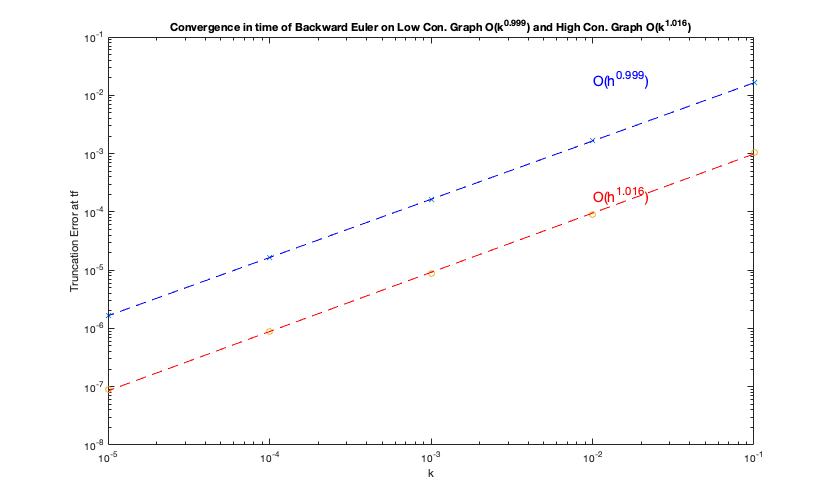
\includegraphics[width=\textwidth]{BackwardEuler.png}
    \end{center}
  \end{figure}





\begin{thebibliography}{3}  % "2" because there are two references

    \bibitem{Simon}
    Cory Simon. (n.d.). \emph{Diffusion on graphs}. Retrieved April 3, 2023, from \href{https://simonensemble.github.io/pluto_nbs/graph_diffusion_blog.jl.html}{https://simonensemble.github.io/pluto\_nbs/graph\_diffusion\_blog.jl.html}
    

    \bibitem{Radu} Horaud, R., \& Horaud, R. (n.d.). A Short Tutorial on Graph Laplacians, Laplacian Embedding, and Spectral Clustering.
  

\bibitem{Poignard} Poignard, C., Pereira, T., \& Pade, J. P. (2017). Spectra of Laplacian matrices of weighted graphs: Structural genericity properties (arXiv:1704.01677). arXiv. \href{https://doi.org/10.48550/arXiv.1704.01677}{https://doi.org/10.48550/arXiv.1704.01677}

\bibitem{leveque}
R.~LeVeque (2007).
\textit{Finite Difference Methods for Ordinary and Partial Differential Equations},
SIAM Press.



\bibitem{spielman} 
Naumann, U.\& Schenk, O. (2012). \emph{Combinatorial Scientific Computing}. CRC Press.



\end{thebibliography}


\end{document}
